\documentclass[tikz,border=3mm]{standalone}
\begin{document}
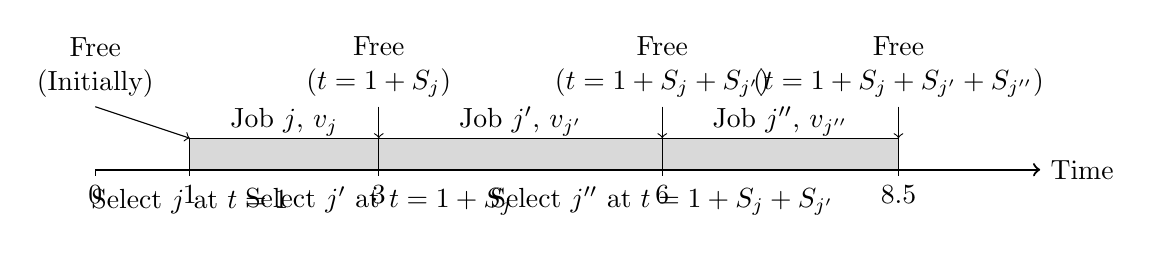
\begin{tikzpicture}[x=1.2cm, y=0.8cm]
% Draw timeline
\draw[thick, ->] (0,0) -- (10,0) node[right] {Time};
\foreach \t in {0,1,3,6,8.5}
  \draw (\t,0) -- (\t,-0.1) node[below] {\t};

% Busy periods (gray filled rectangles)
\draw[fill=gray!30] (1,0) rectangle node[above,midway,yshift=3pt] {Job $j$, $v_j$} (3,0.5);
\draw[fill=gray!30] (3,0) rectangle node[above,midway,yshift=3pt] {Job $j'$, $v_{j'}$} (6,0.5);
\draw[fill=gray!30] (6,0) rectangle node[above,midway,yshift=3pt] {Job $j''$, $v_{j''}$} (8.5,0.5);

% Selection arrows and labels
\draw[->] (0,1) node[above,align=center] {Free\\(Initially)} -- (1,0.5);
\node at (1, -0.5) {Select $j$ at $t=1$};

\draw[->] (3,1) node[above,align=center] {Free\\($t=1+S_j$)} -- (3,0.5);
\node at (3, -0.5) {Select $j'$ at $t=1+S_j$};

\draw[->] (6,1) node[above,align=center] {Free\\($t=1+S_j+S_{j'}$)} -- (6,0.5);
\node at (6, -0.5) {Select $j''$ at $t=1+S_j+S_{j'}$};

\draw[->] (8.5,1) node[above,align=center] {Free\\($t=1+S_j+S_{j'}+S_{j''}$)} -- (8.5,0.5);
\end{tikzpicture}
\end{document}